% \documentclass[a4paper,twoside]{memoir}
\documentclass[a4paper,twoside,oldfontcommands]{memoir}
\usepackage{graphicx}
\usepackage{url}
\usepackage{siunitx}
\usepackage{natbib}
\usepackage{har2nat}
\usepackage{GoudyIn,lettrine}
\renewcommand\LettrineFontHook{\GoudyInfamily}
\newcommand{\URL}[1]{$\langle$\url{#1}$\rangle$}
\DeclareOldFontCommand{\bf}{\normalfont\bfseries}{\mathbf}
% This is the chapter titled `Optical TEMPEST' in Ireneusz Kubiak's new book.
\begin{document}
\title{New Book}
\author{Joe Loughry}
\setcounter{chapter}{6} % This chapter will be Chapter 7 of the book.
\setcounter{page}{262} % Page 263 will be the first page of this file.
\thispagestyle{empty}
\chapter{Optical TEMPEST}
\lettrine[lines=3]{T}{he} leakage of information from a system through a
channel of modulated light is a vulnerability. The operative terms are `leakage',
`information', `channel', and `modulated light'. The \emph{leakage} might be
accidental or it might be caused on purpose by an adversary, but it is not
supposed to be there. \emph{Information} can be anything from a single bit to
large volumes of information; it might be extremely valuable information like
cryptographic keys. \emph{Channels} in the Shannon sense \cite{Shannon1948}
have a bandwidth-delay product, and noise; both of these are important to
understand the risk of optical TEMPEST. And finally, \emph{modulated light}
carries the signal. Light can be modulated in time or in space---here we think of
light modulated in the time domain. Light modulated in the space domain is an
\emph{image}; `shoulder surfing' is a real risk but not the one we are
concerned with here.\footnote{\emph{Shoulder surfing} is the clandestine
surveillance of display screens or keyboard activity for the purpose of
stealing secrets. It might be done visually or through a video camera; it can
even be done without line-of-sight, by deconvoluting a distorted reflection off
a shiny object in the optical path
\cite{Backes2008,Backes2009a,Raguram2011,Jenkins2013a,Xu2013a}.}

Further in the time domain, light can be amplitude-modulated, or
frequency-modulated, or phase-modulated. Of the three possibilities, amplitude
modulation (AM) is the most plausible for optical TEMPEST (from a physical
standpoint) because optical TEMPEST vulnerabilities most often depend on the
accidental or improvised existence of a modulated---or modulatable---channel,
and AM is likely the simplest and most straightforward to implement. On-off
keying (OOK) is the simplest AM method and the most likely to occur
accidentally; in OOK, light \emph{on} means a binary 0 or 1, and light
\emph{off} means the other kind. OOK is not self-clocking: the receiver must
know {\it a priori} or be able to figure out the sender's intended \emph{bit
interval} to decode the signal; there are better \emph{line codes} than OOK
that a deliberate sender inside the target system may be able to
use---Manchester coding, for example---but most often the adversary is limited
to exploiting sources and methods that are already there.
\subsection{Light Sources}
Compromising emanations take one of two paths: they may be \emph{conducted} or
\emph{radiated}. Light sources vulnerable to optical TEMPEST include visual
indicators---a subset of which are video displays---and discrete indicators. If
controlled automatically, indicators are not as useful as if they may be set by
the adversary.

Figure \ref{figure:taxonomy} shows the taxonomy of optical TEMPEST in the
larger context of vulnerabilities due to \emph{compromising
emanations}---exploitable leakage of measurable physical phenomena out of a
system that can be interpreted by an adversary to gain information about the
internal state of the system.
\begin{figure}[h]
  \centering
  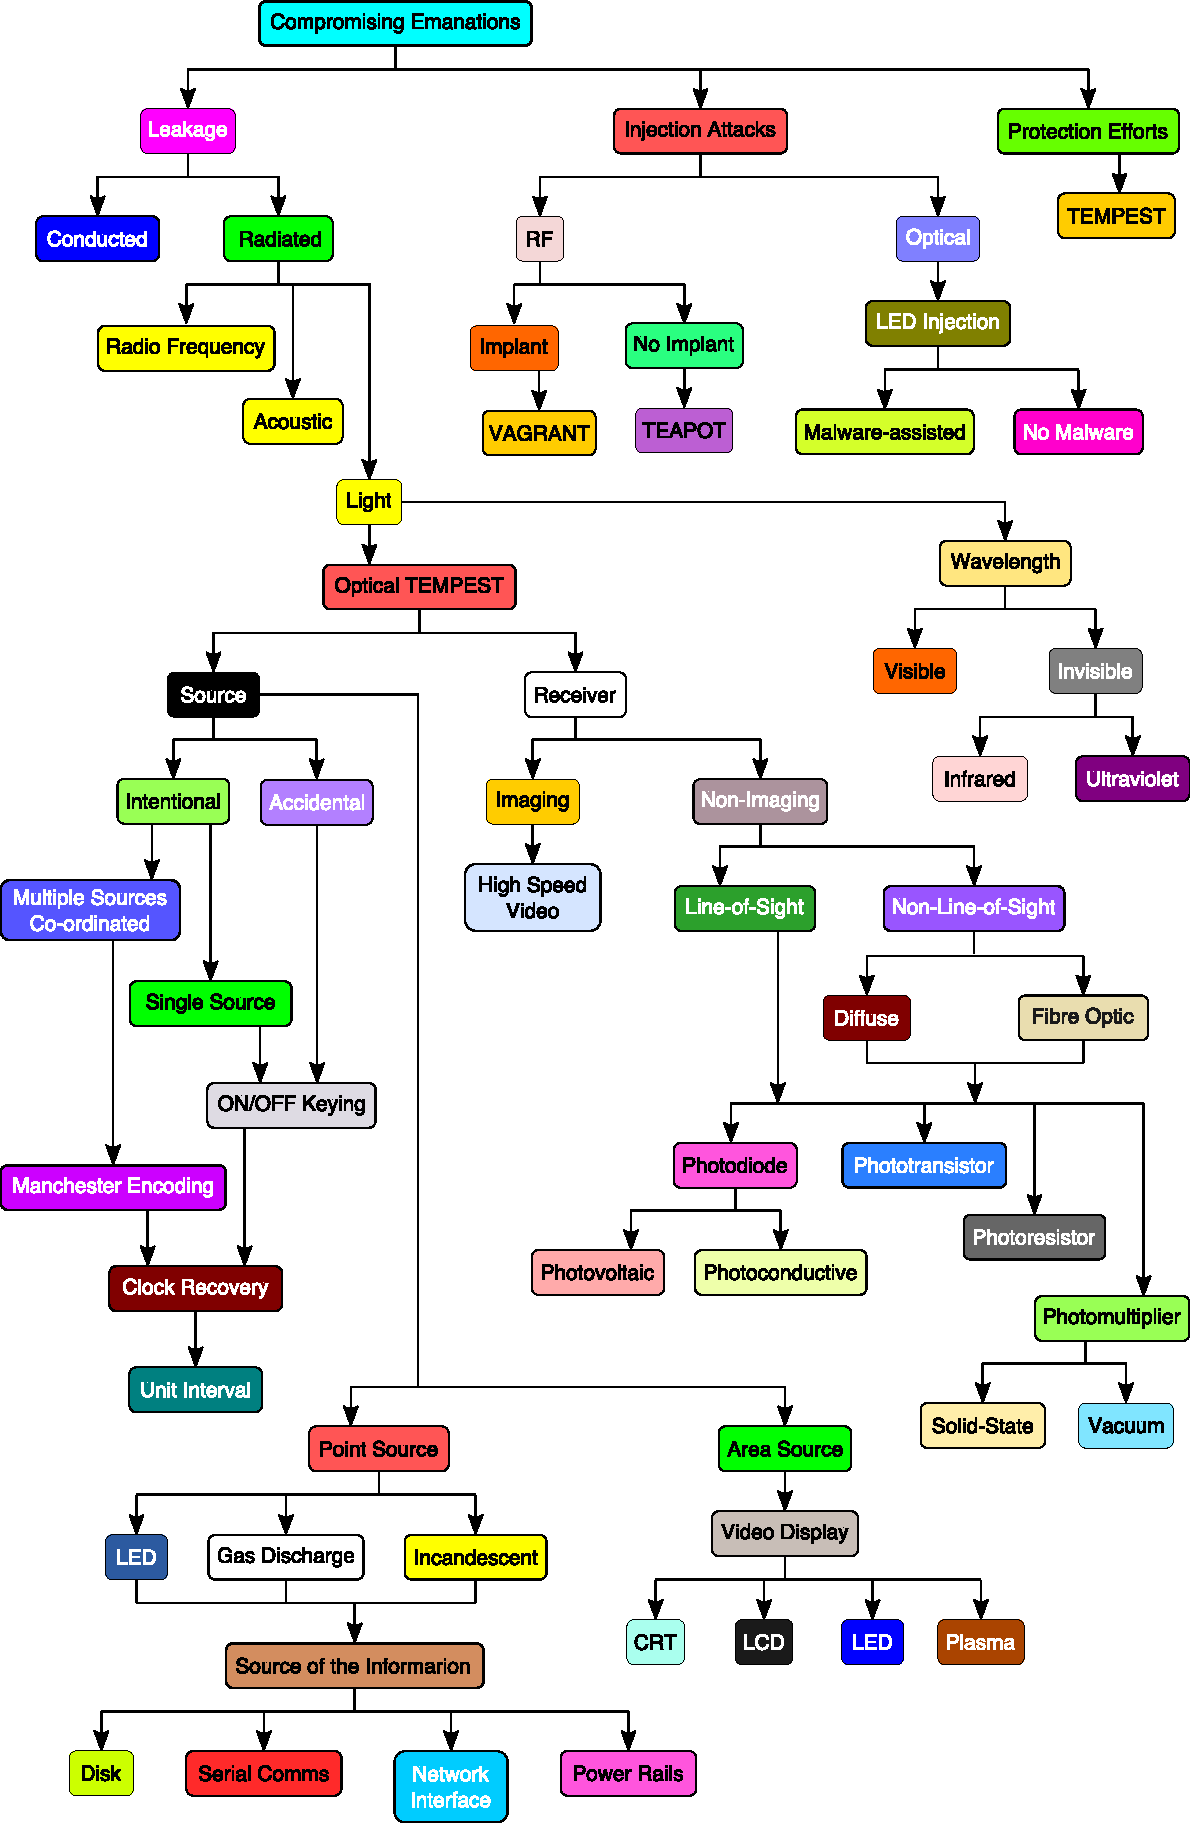
\includegraphics[width=\textwidth]{taxonomy.pdf}
  \caption{Taxonomy of compromising emanations.}
  \label{figure:taxonomy}
\end{figure}
\subsection{Sensors}
Given these sources of compromising emanations (accidental or intentional), to
have a communication channel there must be a receiver. Many kinds of optical
sensors will suffice, but what is needed particularly is an optical sensor with
a fast response time. Photodiodes, photomultipliers (solid state or otherwise),
phototransistors, photoresistors, or even some video cameras might be used.
Still cameras are not suitable.
\subsection{Induced Emanations}

\subsection{The clock recovery problem}

(Figure from 2002 paper)

Depending on the nature of the leakage, information leakage through optical
emanations may or may not be a covert channel. By the classical definition,
due to \cite{Lampson1973}, a covert channel is made of a pair of communicating
processes, but in many cases, the source of compromising optical emanations
is in hardware, not a programme running on the CPU.

electromagnetic but in the optical spectrum; we consider that to include at
least infrared (wavelengths longer than \SI{700}{\nano\metre}) because of the
ubiquitousness of light emitting diode (LED) sources in that range and their
convenient invisibility to humans.

\sidebar{\centerline{\textbf{How dangerous?}}\medskip
\textbf{Class I} optical emanations are correlated only minimally with the state
of a device; they tell if it is on or off. \textbf{Class II} emanations leak
information about the activity level of a device---is it busy or idle?
\textbf{Class III} optical emanations are correlated with the contents of data,
and are extremely hazardous.}

Cite \cite{Allain2019}.

\section{History}
The U.S.\ National Security Agency (NSA) named TEMPEST, as far as we know. We
don't even know for sure that the word is not an acronym. It is believed to
be a code name, \textsc{Tempest}\footnote{Evidence for it is shaky but there
was supposedly another programme called \textsc{Teapot} dealing with
stimulated RF compromising emanations \cite[p.~539]{Anderson2008a} and
partially corroborated in December of 2013 by Edward Snowden (NSA ANT
catalogue).} but evidence in the open literature is scarce; the only clear
original source is one declassified document dating from 1972 in which
everything related to emanations other than RF is redacted
\cite{NSAtempest2007}.
\subsection{Information Leakage}
\subsubsection{Electromagnetic}
Field telephones in WWI; \emph{funkspiel} in WWII; electromechanical cypher
machines in West Berlin. (This topic is covered well elsewhere in the book.)
\sidebar{\centerline{\textbf{Video Cameras}}\medskip
It is tempting to think of using video cameras to capture an entire rack of LED
indicators at once, but that won't work. The reason is because video cameras
have a relatively low \emph{frame rate}---usually 30--240 frames per
second---and this is not fast enough to capture the transitions we're
interested in.}
\subsection{TEMPEST}
The protection of information from remote eavesdropping; air gaps; control
zones; protected distribution systems (PDS)\footnote{Visibility, stories of
poison gas, flammable gas, pressure gauges---reference Anderson (2001).} The
inclusion of acoustic but overlooking of optical, with the exception of
shoulder surfing. Contextual blindness?
\subsection{Optical}
LEDs and CRTs---Figure \ref{figure:slow-mo_guys_crt}.
\begin{figure}[ht]
  \centering
  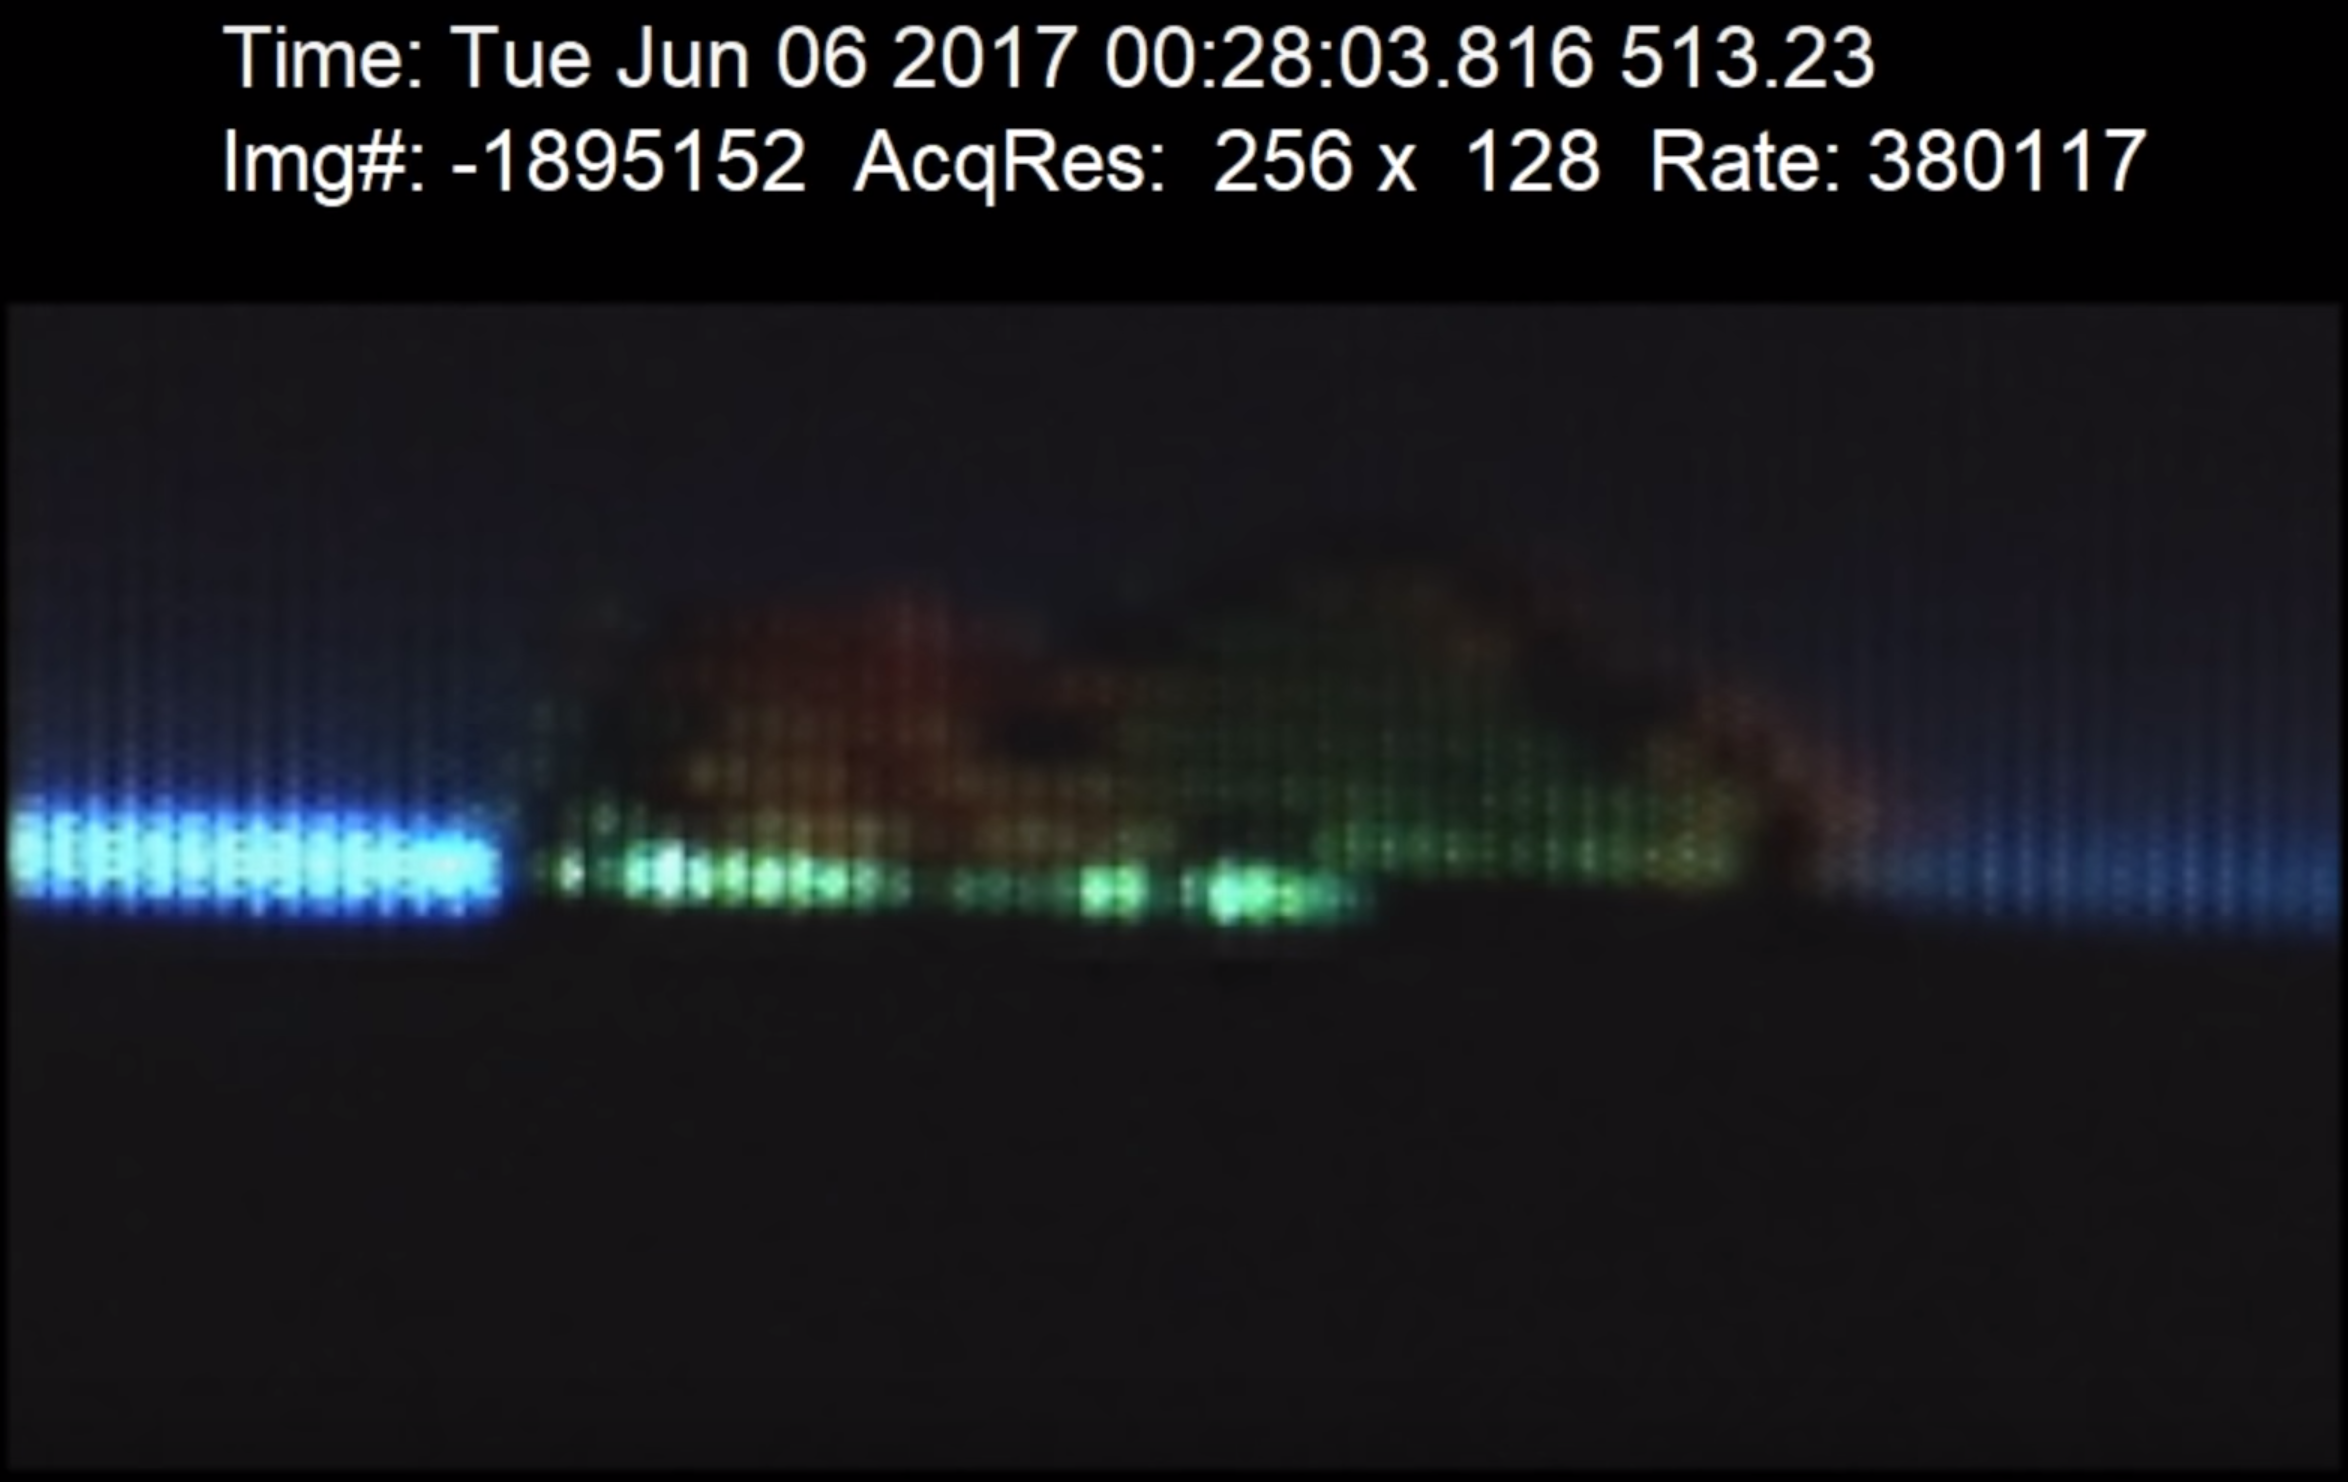
\includegraphics[width=3in]{slow-mo_guys_crt.png}
  \caption{High speed camera image (380\,117 frames per second) of CRT electron
    beam exciting phosphor dots \protect\cite{Free2018}.}
  \label{figure:slow-mo_guys_crt}
\end{figure}
\section{Physical Principles}
Photons, energy, generation atmospheric absorption. Recent development of
high efficiency LEDs (and the unexpected effect that had on reversing LEDs).
Telescopic optics, fibreoptic collection.
\begin{figure}[ht]
  \centering
  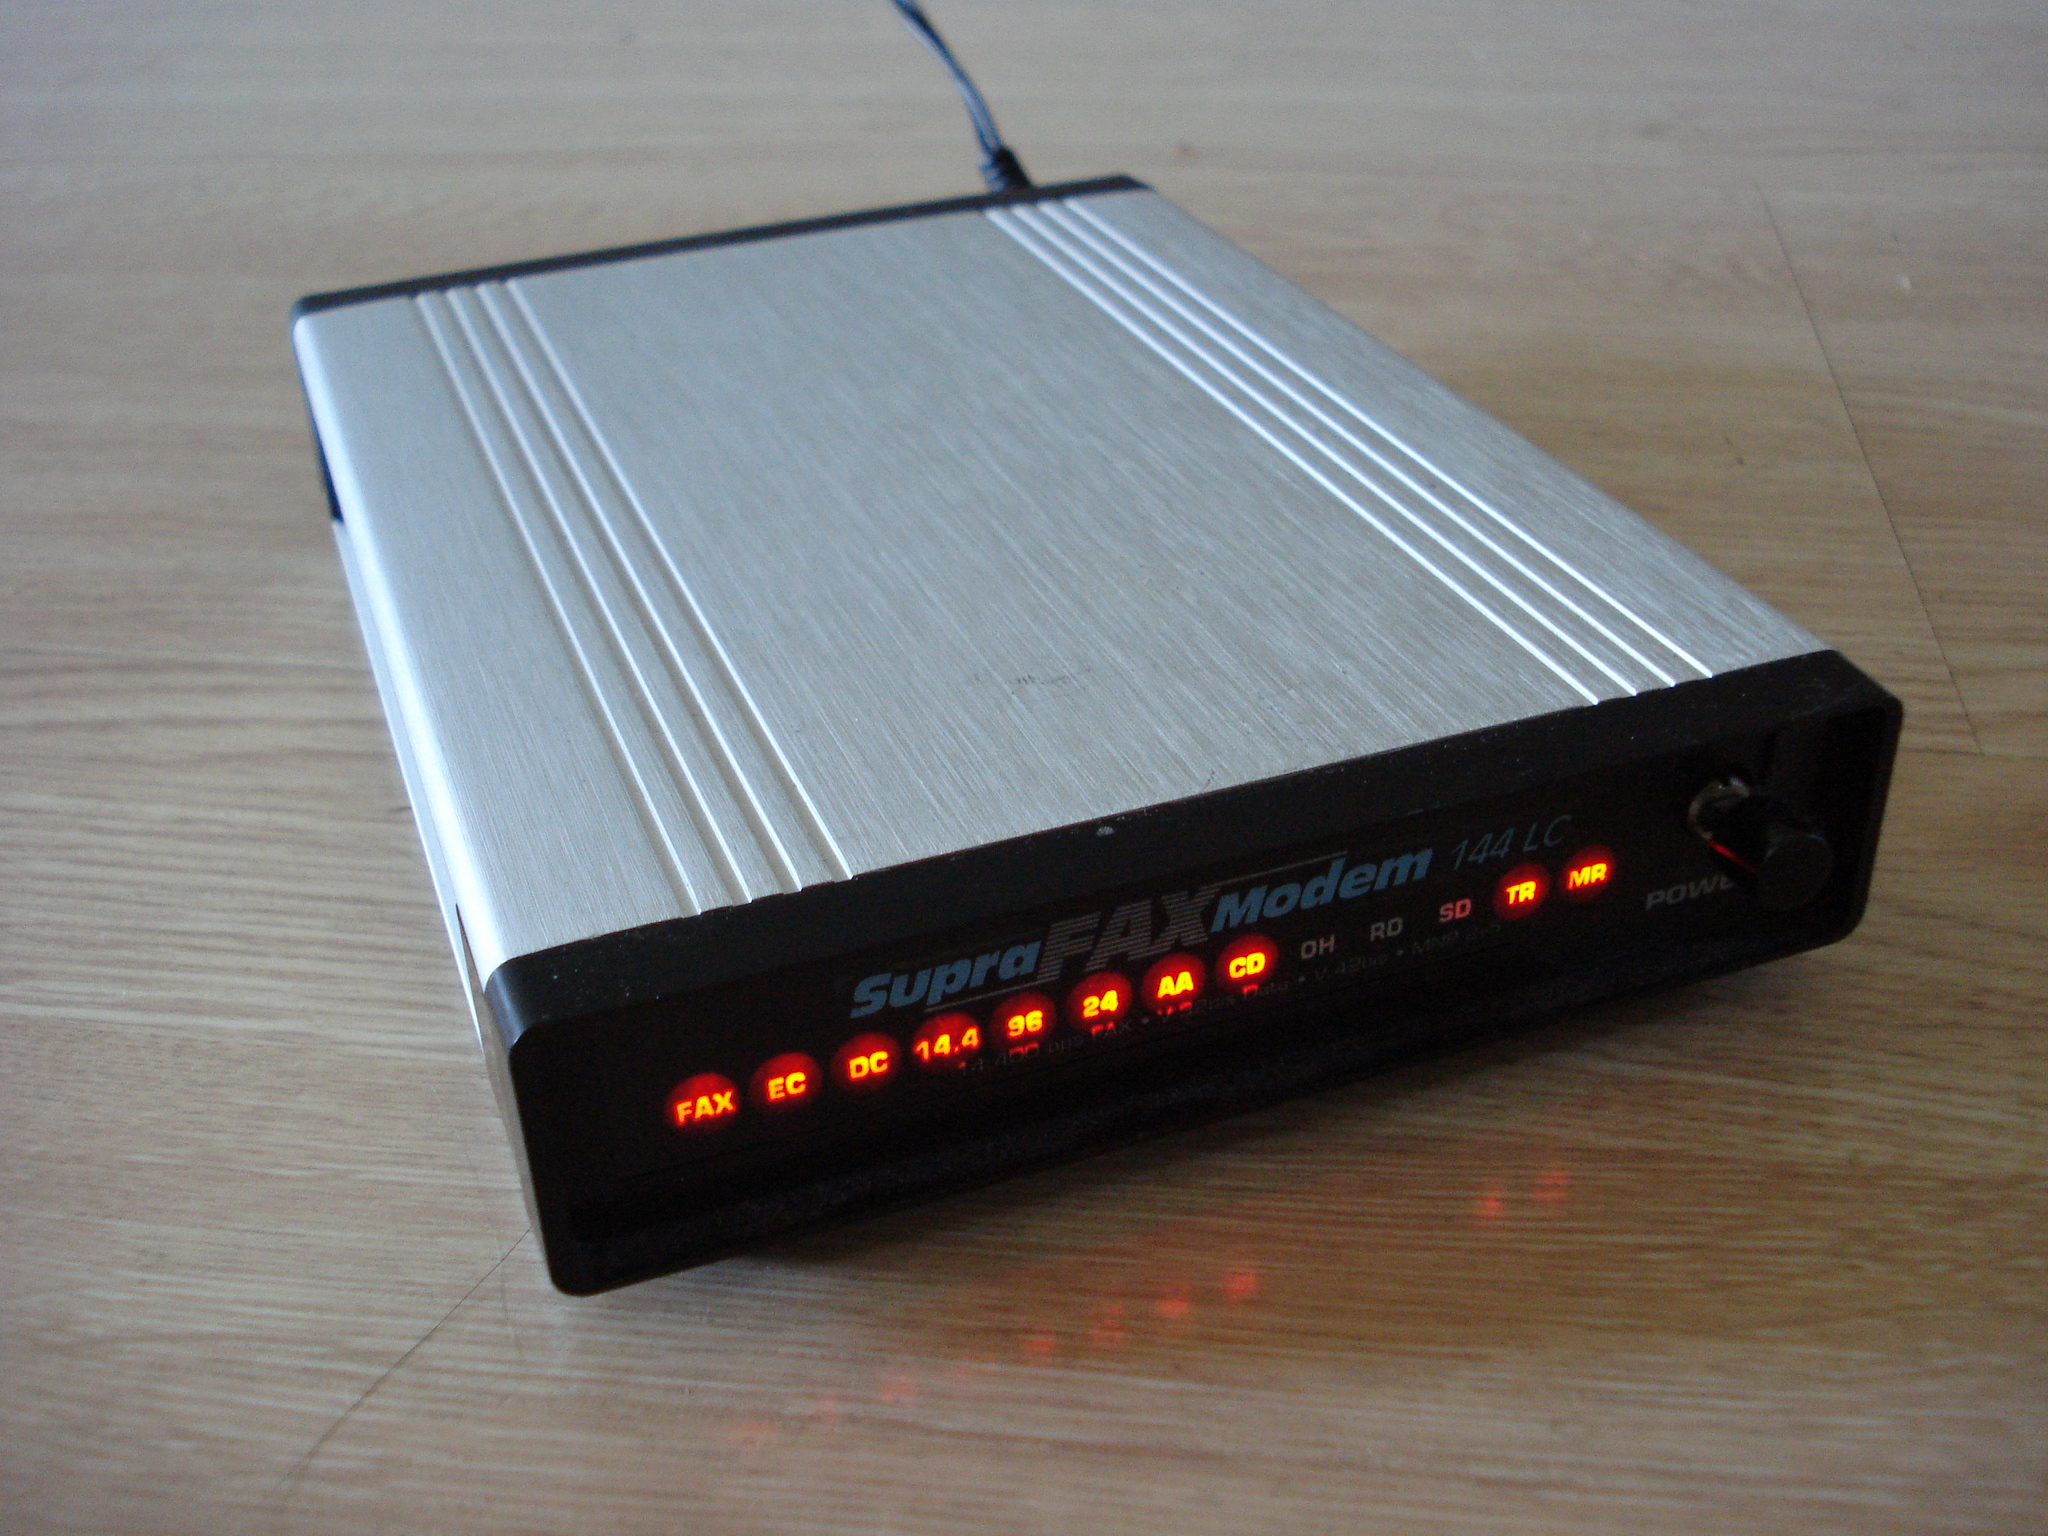
\includegraphics[width=3in]{SupraFAXmodem_144_LC_photo_courtesy_Wikipedia.jpg}
  \caption{Some LED indicators leak information.}
  \label{figure:modem}
\end{figure}
\subsection{The Unreasonable Effectiveness of Signal Processing}
One surprising thing, to anyone unfamiliar with digital signal processing, is
how effectively it can pull a usable signal out of what appears to be
hopelessly noisy data. An example may be seen in Fig.\ 4 of
\cite{Loughry2002a}.

Need a new figure here.

\section{Current Research}
Guri \emph{et al.} But they are covert channels. But these are covert
channels. Difference between covert channels and side channels
(ref.\ Kocher).
\subsection{Resurgence of Interest 201?--present}
Aside from the `Compromising Reflections' paper, not much happened until
around 2010, except for\ldots\footnote{Parts of this section was presented at
EMC Europe 2018, in Amsterdam, the Netherlands (\emph{International Symposium
and Exhibition on Electromagnetic Compatibility}), 27--30 August 2018
\cite{Loughry2018a}.}
\subsection{Perspective}
It's not only LEDs; and LEDs are not only used as status indicators; Figure:
\emph{all} the information channels in and out of a PC---or more accurately,
an information processing system. A new conception of control zone;
Robinson's `energy gap' concept and its applicability to crypto.
\section{Future Directions}
Unpublished research
\subsection{LED Reversing}
Recent research---as yet unpublished---extends the idea of information leakage
through LEDs in the other direction. Unintended photosensitivity of junction
semiconductor devices has been known since at least the nineteen-seventies;
UV-eraseable programmable read-only memory (EPROM) chips take advantage of the
fact. Mims \citeyear{Mims1973b} was first to note in print that LEDs work as
photodiodes, both in the forward-biased (photovoltaic) and reverse-biased
(photoconductive) modes.

Would an unmodified LED, with leads splayed out, act as a WiFi powered
optical bug? Could a \SI{5}{\giga\hertz} WiFi illumination power it in
\emph{reverse bias} photoconductive mode to turn it into an optical RF
modulator? It's a nonlinear junction (diode) detector already---but can
incident \emph{optical} radiation modulate through the diode the reflection
from the leads of the ambient microwave interrogation carrier?

Modern microprocessors do not expose their address and data bus lines as
earlier ones did. But what happens when LEDs on external pins (whether
configured for output, by the system designer, or reconfigured for input by an
attacker) drive those pins unexpectedly?
\begin{figure}[ht]
  \centering
  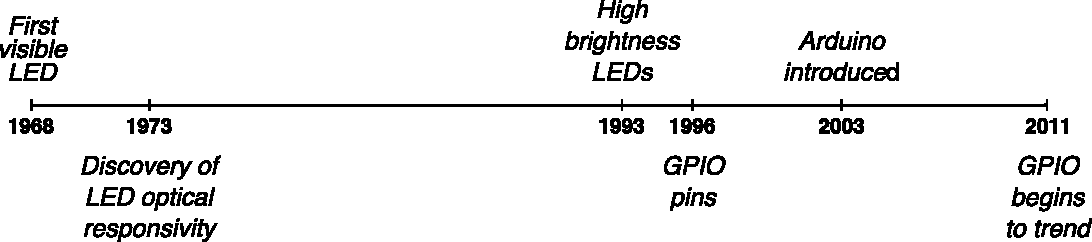
\includegraphics[width=\textwidth]{timeline.pdf}
  \caption{Confluence of several technological developments made reversing LEDs
    possible.}
  \label{figure:timeline}
\end{figure}
first visible LEDs for indicators in 1968 (Figure \ref{figure:timeline}).
photoresponsivity of LEDs in 1973
first high brightness LEDs used in 1993
GPIO in 2011 (Google Trends) although the concept dates to Intel 8255 and MOS
6522. The Atmega8 used by Arduino introduced programmable pull-up and pull-down
resistors in 1996 \cite{Mims1973b,Atmel2013,Stringfellow1997}.

External hardware pull-up or pull-down resistors, as on the Intel 8255 and MOS
6522 chips used in the 1980s, were of course inaccessible to an adversary; CMOS
variants of the 8255 had internal pull-up resistors but they were not
programmable. (Automatically configured pull-up or pull-down resistors may be
considered a special case of external discrete hardware components.)
\begin{figure}[ht]
  \centering
  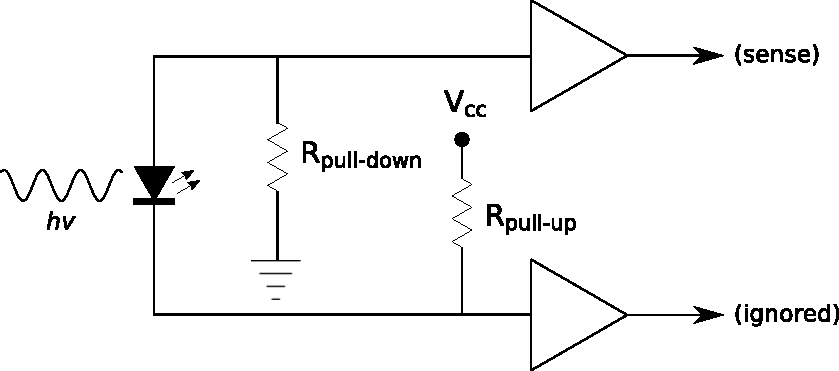
\includegraphics[width=2in]{nonsensical.pdf}
  \caption{Programmable pull-up and pull-down resistors can be abused by
    setting them in non-sensical ways, such as this, to reverse-bias an LED
    and sense it---as a photodiode---in the (much faster) photoconductive
    mode.}
  \label{figure:nonsensical}
\end{figure}
Programmable pull-up and pull-down resistors, introduced in 1996 with the
ATmega8 microcontroller \cite{Atmel2013} are far more useful to an adversary
adversary because they can be set in nonsensical ways (Figure
\ref{figure:nonsensical}).\footnote{The trick only works if the designer chose
to save a power pin by connecting an LED to a pair of GPIO pins, which might
make sense if unused GPIO pins happen to be available.}

\emph{Cf.}\ Snowden's disclosures of NSA's TAO catalogue, for a certainty.
\subsubsection{Classical covert channels}
\subsubsection{Dead blow hammer}

\section{Bell's Inequality}
For the \SI{33}{\pico\second} interval between those two points, the light does
not exist in this universe.

Bell's Inequality \cite{Bell1964}.
\bibliographystyle{agsm}
\bibliography{consolidated_bibtex_file}
\end{document}
